\section{Introduction}

When reading a scientific article, the reader's comprehension of the text may
be greatly improved by inclusion of charts, tables and figures that help summarise information.
For example, in \figref{table-explanation}, findings from climate change models
are summarized in a table with an accompanying paragraph providing the reader
with context for interpeting the table, references to ``SSP-'' in the text meaning
the rows of the table, with column of interest left implicit at first.

Visualizations such as tables and bar-charts summarize data to make it easier to
understand. The readers comprehension can be further aided by incorporating 
interactivity into the visualization. By enabling the reader to click on parts
of a chart to see the data it summarizes, the reader gets a better sense of what
the author is trying to say. Understanding can be improved further, by extending
interactivity to the text itself.

Authoring of such articles is already difficult and time-consuming, and asking
the author to build in interactive features is unreasonable. As yet, there are
no tools that treat supporting text as a visual element to interact with. It is
not entirely clear what interactive text might look like. 

Some of the difficulty can be mitigated by building visualizations in a language
which provides automatic support for interaction, but these do not provide tools
or support for linking data directly to the text of an article. An article will
be full of references to items of discourse, and asking the author to manually
link each reference to its referent for the purposes of interaction is liable to
error, or the user simply giving up. An automated tool is required. 

\begin{figure}
   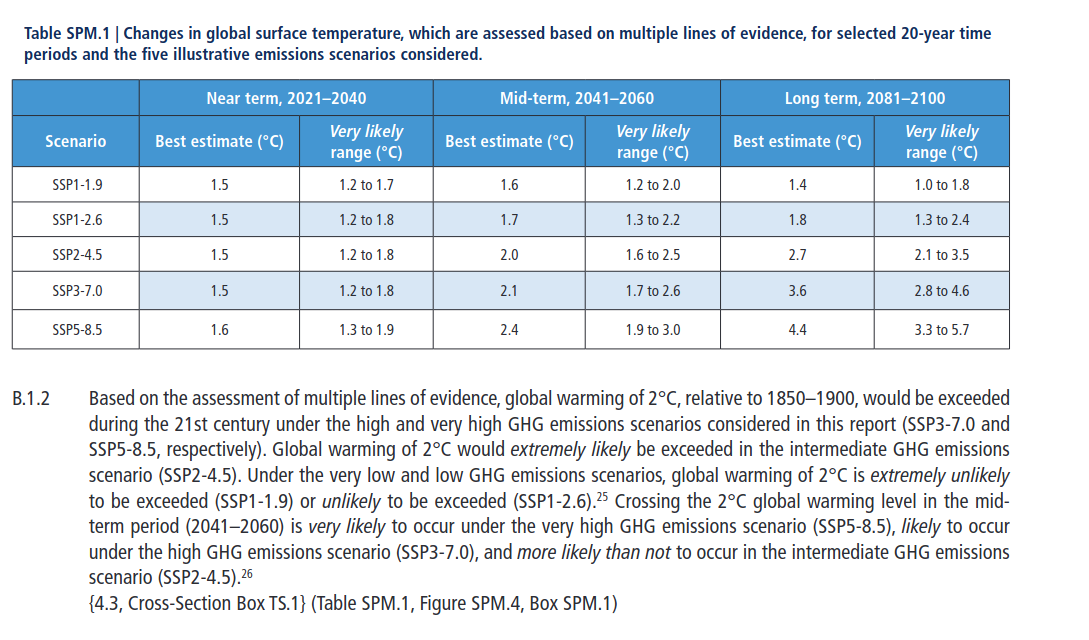
\includegraphics[width=0.9\textwidth]{fig/ipcc-table-explanation.png}
   \caption{Explanation based on the contents of a table}
   \label{fig:table-explanation}
\end{figure}